\documentclass[11pt,a4paper]{article}
\usepackage[a4paper, margin=3cm]{geometry}
\author{
 Shan Eapen Koshy
}
\usepackage{tikz}
\usepackage{makecell}
\usetikzlibrary{shapes}
\usepackage{mathtools}
\usepackage{amsmath}
\DeclarePairedDelimiter\ceil{\lceil}{\rceil}
\DeclarePairedDelimiter\floor{\lfloor}{\rfloor}

\begin{document}
\title{Min And Max Height of a B-Tree}
\maketitle

\section{Introduction}
A B-Tree is a generalization of binary search tree in which a node can have more than two children. The maximum number of children the B-Tree can have is specified by its order. A B-Tree of order m can have m-1 keys in each node.
So by using the definition of a B-Tree, we are interested in determining the minimum and maximum height given the order m and total number of keys n.


\section{Minimum Height}
The minimum height of B-Tree is obtained when all the nodes are completely filled. Now let's calculate the total number of keys. 
\\\\Max number of keys
\begin{align*}
&= (m-1) + m(m-1) + m^2(m-1) + ... + m^h(m-1)\\
&= (m-1)\{1+m+m^2+...+m^h\}\\
&= (m-1).1\frac{m^{h+1}-1}{(m-1)}\\
n &= m^{h+1}-1
\end{align*}
To find the minimum height, we rearrange the equation as given below
\begin{align*}
n+1 &= m^{h+1}\\
h+1 &= \ceil{log_m (n+1)} \\
h_{min} &= \ceil{log_m (n+1)}-1
\end{align*}

Given below is an example of a B-Tree of order 3 and 8 key elements. The tree has a height of 1 (considering root as 0) which is satisfied by the equation
\begin{align*}
h_{min} &= \ceil{log_3 {(8+1)}}-1 \\
h_{min} &= 2-1 \\
h_{min} &= 1
\end{align*} 

\begin{center}
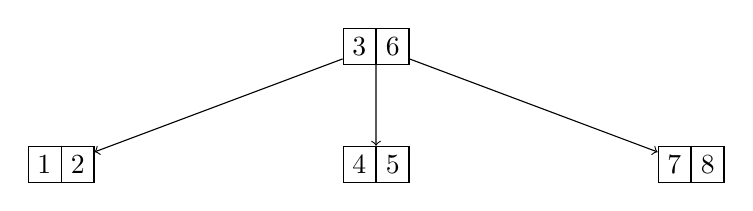
\begin{tikzpicture}
\tikzstyle{bplus}=[rectangle split, rectangle split horizontal,rectangle split ignore empty parts,draw]
\tikzstyle{every node}=[bplus]
\tikzstyle{level 1}=[sibling distance=40mm]
\tikzstyle{level 2}=[sibling distance=15mm]
\node {3 \nodepart{two} 6} [->]
  child {node {1 \nodepart{two} 2}} 
  child {node {4 \nodepart{two} 5}} 
  child {node {7 \nodepart{two} 8}} 
;\end{tikzpicture}
\end{center}




\section{Maximum Height}
To obtain maximum height of the B-tree, we have to fill each node with the minimum number of keys and by maintaining the B-tree properties. That is, each node should contain atleast \ceil[\Big]{\frac{m}{2}} keys.

Take d = \ceil[\Big]{\frac{m}{2}}
\par Consider the table below
\begin{center}
 \begin{tabular}{||c c c ||} 
 \hline
 Height & Min no of nodes & Min no of keys \\ [2.5ex] 
 \hline\hline
 0 & 1 & 1  \\ [2ex] 
 \hline
 1 & 2 & \makecell{2(\ceil{\frac{m}{2}}-1)\\= 2(d-1)} \\ [2ex] 
 \hline
 2 & 2d & 2d(d-1)  \\ [2ex] 
 \hline
 3 & 2d^2 & 2d^2(d-1)  \\ [2ex] 
 \hline
 .. & .. &  .. \\ [2ex] 
 \hline
 h & 2d^{h-1} & 2d^{h-1}(d-1)  \\ [2ex] 
 \hline
\end{tabular}
\end{center}

\\\\Min number of keys
\begin{align*}
&= 1 + 2(d-1) + 2d(d-1) + 2d^2(d-1) + ... + 2d^{h-1}(d-1)\\
&= 1 + 2(d-1)\{ 1 + d + d^2 + ... + d^{h-1}\}\\
&= 1 + 2(d-1) \{\frac{d^h-1}{(d-1)}\}\\
&= 1 + 2(d^h-1)\\
&= 1 + 2\ceil[\Big]{\frac{m}{2}}^h-2\\
n &=  2\ceil[\Big]{\frac{m}{2}}^h-1
\end{align*}
To find the maximum height h of the B-Tree we can simply rearrange the equation
\begin{align*}
\ceil[\Big]{\frac{m}{2}}^h&= \frac{n+1}{2}
\\h &= \floor{log_{\ceil{\frac{m}{2}}} \frac{n+1}{2}}
\\h_{max} &= \floor{log_d \frac{n+1}{2}} , where \ d = \ceil{\frac{m}{2}} 
\end{align*}

The B-Tree shown below has the same number of key elements and has order 3. The tree is drawn such that it has maximum possible height i.e 2 in this case.
\begin{align*}
\\h_{max} &= \floor{log_2 \frac{8+1}{2}} , where \ d = \ceil{\frac{m}{2}} = 2 
\\ &= \floor{2.169}
 \\&= 2 
\end{align*}

\begin{center}
\begin{tikzpicture}
\tikzstyle{bplus}=[rectangle split, rectangle split horizontal,rectangle split ignore empty parts,draw]
\tikzstyle{every node}=[bplus]
\tikzstyle{level 1}=[sibling distance=60mm]
\tikzstyle{level 2}=[sibling distance=15mm]
\node {4} [->]
  child {node {2 \nodepart{two} }
    child {node {1 \nodepart{two}}}  
    child {node {3 \nodepart{two}}}   
  } 
  child {node {6 \nodepart{two} }
    child {node {5 \nodepart{two}}}    
    child {node {7 \nodepart{two}}}    
  }
;\end{tikzpicture}
\end{center}


\end{document}